
\chapter{blockchain}
\label{blockchain}
Consensus protocols that work with Byzantine-failure nodes and allow open membership are used in open blockchains. By an open blockchain we understand one where nodes can freely join the network and participate in the consensus protocol. Examples of such blockchains are Bitcoin \cite{nakamoto2008peer}, Ethereum \cite{wood2014ethereum}, and Stellar \cite{mazieres2015stellar}. Bitcoin uses a proof-of-work consensus algorithm where the computational power dictates the contribution to the consensus decision. Ethereum plans to switch to a proof-of-stake consensus where the amount of cryptocurrency dictates the contribution to the consensus decision. Stellar uses Federated Byzantine Agreement where the trust dictates the contribution to the consensus decision. We decide to use the last one, and the rationale for doing so is described in Sec. \ref{FBA}.

Data stored in a blockchain are immutable––once written, they cannot be changed. Data are also secure against the intruders (as long as they do not control most of the consensus means). Data types differ in different blockchains, most of which store transactions to update a global ledger. Some blockchains, like Ethereum, also allow storing smart contracts\footnote{Smart contracts are scripts that are executed on virtual machines on all nodes and use blockchain as a persistent storage}, though we do not see any benefit of using them in our system. We use a simple transaction model with a slight modification that prevents pre-signing of proof-of-time transactions. A full description is provided in Sec. \ref{blockchain-structure}.


\section{System proposition}
We propose a system where all or part of the nodes in the ICN network participate in a blockchain consensus protocol––securely storing a common database consisting of proof-of-time claims, along with the Content Store. Each node can be sure that the rest of the network stores the same version of the blockchain database. But the most vital feature of our system is that by using a blockchain, we ensure that publishers can publish only one proof-of-time at a time. Therefore, to authenticate the content, they must prove their access to credentials over a long enough period of time, unaffordable for a malicious publisher but affordable for an honest one. This is the statement we base our authentication mechanism on. A publisher wishing to confirm content authenticity must submit a carefully prepared transaction to the blockchain network. The transaction––a proof-of-time claim––must include:
\begin{itemize}
    \item A hash of the content to authenticate.
    \item A signature on the claim that proves access to appropriate credentials.
    \item The publisher's public key used to verify the signature and identify the publisher.
    \item A hash of the previous block to prevent pre-signing of transactions.
\end{itemize}
A graphical illustration of such a transaction is presented in Fig. \ref{fig:proof-of-time}.
\begin{figure}[h!]
    \centering
    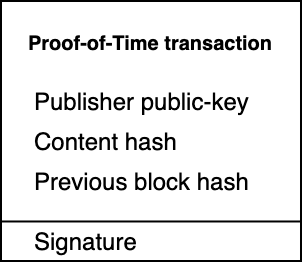
\includegraphics[width=0.4\textwidth]{img/proof-of-time_transaction.png}
    \caption{Structure of proof-of-time claim}
    \label{fig:proof-of-time}
\end{figure}

The publisher submits the transaction to the nearest node, which includes it in a block and broadcasts to the rest of the network. Once all network nodes approve the block (through the consensus protocol described in Sec. \ref{FBA}), the publisher can create the next proof-of-time transaction pointing to the previous block's hash. The process is repeated until the required Credibility Score (described in Sec. \ref{credibility-score}) is reached. In the sequel, we describe the details of the system based on blockchain.

\section{Blockchain layer}
In our proposal, network nodes play two roles: of an ICN node participating in routing and content caching, and of a blockchain node participating in the consensus protocol and blockchain storage (see Fig. \ref{fig:combined_layers}). Not every node has to play these two roles--the ones not connected to end-users might not participate in the blockchain, since they do not claim content trustworthiness. 
The blockchain layer could also be managed by entities other than network nodes, thus separating the content distribution (transport) layer from the trust layer, cf. Fig. \ref{fig:separated_layers}. The ICN nodes could be relieved from the trust network overhead, which could make them simpler. Also, the trust system would be more portable; it could be used in different ICN solutions, and even in legacy systems, since the developed trust does not depend on the ICN architecture but on the hash of the content and publisher credentials. The blockchain trust network could be hosted by more powerful devices and possibly different organizations––achieving separation of concerns, which is always desirable in the long term. For the rest of the thesis, we assume the separation of roles (ICN and blockchain), but the decision if one node should play one or two roles is up to the implementation.
\begin{figure}[h!]
\centering
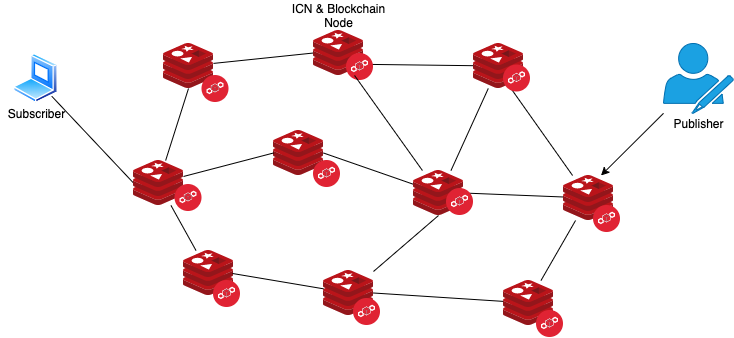
\includegraphics[width=1\textwidth]{img/combined-layers.png}
\caption{Combined layers}
\label{fig:combined_layers}
\end{figure}

\begin{figure}[h!]
\centering
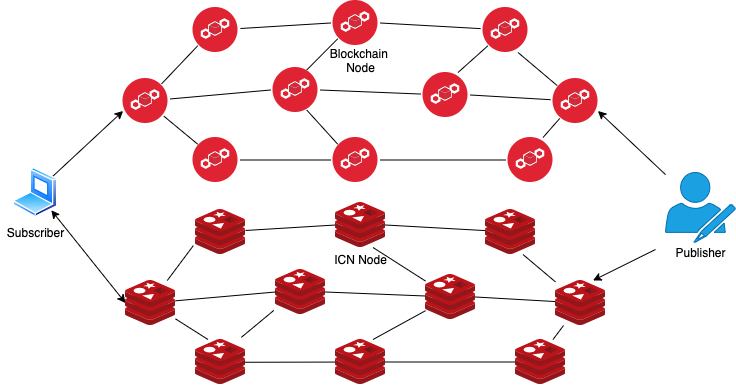
\includegraphics[width=1\textwidth]{img/separated-layers.png}
\caption{Separated layers}
\label{fig:separated_layers}
\end{figure}

\section{Credibility Score}
\label{credibility-score}
In the GI protocol, there are two states of content authenticity: authenticated and not-authenticated. We believe that this is limiting. Content like, e.g., weather forecasting, should not be authenticated for the same amount of time as data in a banking website. Therefore we propose a more flexible model, where authentication can be acquired progressively via Credibility Score, mentioned in Section \ref{proof-of-time}, which increases authentication granularity. Different thresholds should be used for different content types. For example, if three trust thresholds are used: low, medium, and high; then, we can require 10 minutes, 2 hours, and 12 hours of proof-of-time respectively. Each time the content is published to the network with stolen credentials, their owner can be notified about it, and has a certain time to revoke the credentials and halt the malicious authentication process.

\section{Publisher flow}
A publisher wishing to publish content on the ICN network and then authenticate it over the blockchain network needs to take the following steps:
\begin{enumerate}
    \item Create a Named Data Object (NDO), which requires signing the content using the publisher's key pair.
    \item Compute a hash of the NDO.
    \item Create a proof-of-time transaction, which includes the hash of the NDO, hash of the previous blockchain block, and the signature proving access to the private key.
    \item Publish the proof-of-time transaction to the blockchain node.
    \item Repeat steps 3 and 4 until the Credibility Score is reached.
\end{enumerate}
The complete flow of publishing the content to the ICN node and blockchain node is presented in Fig. \ref{fig:distribution-flow}
\begin{figure}[h!]
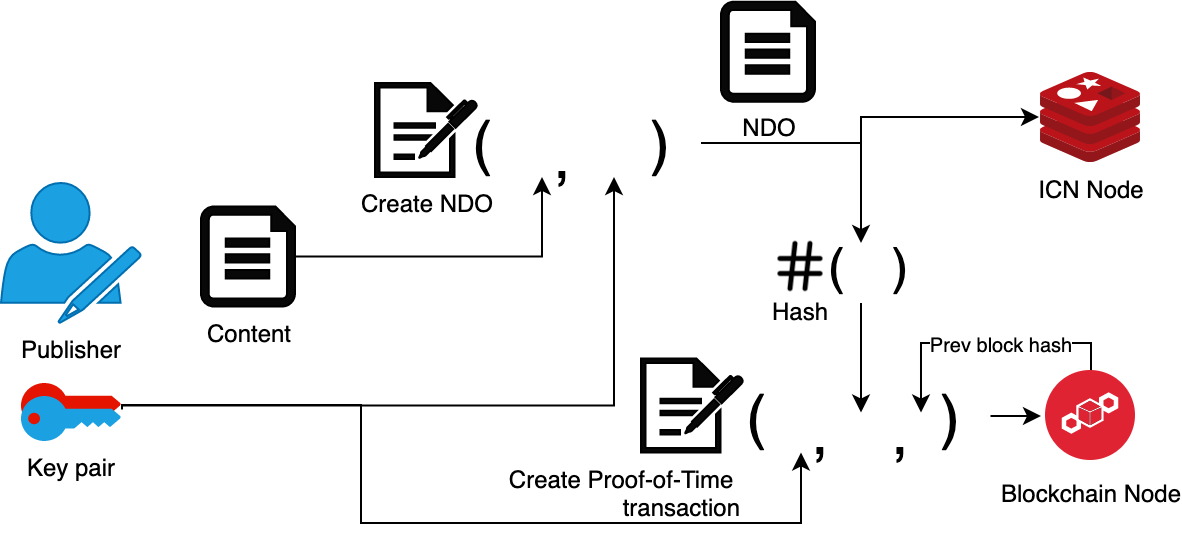
\includegraphics[width=9cm]{img/distribution-flow.png}
\centering
\caption{Flow of publishing content to ICN and proof-of-time to blockchain}
\label{fig:distribution-flow}
\end{figure} 

\section{Subscriber flow}
A subscriber willing to fetch the content from the ICN network and verify the authenticity from the blockchain has to take the following steps:
\begin{enumerate}
    \item Send an Interest packet with a content name to the nearest ICN node.
    \begin{itemize}
        \item subsequently, the ICN node returns a Data packet with content, signature, and the publisher's public key.
    \end{itemize}
    \item Send a Credibility Score request along with the hash of the content and the publisher's public key to the blockchain node.
    \begin{itemize}
        \item subsequently, receive the Credibility Score from the blockchain node.
    \end{itemize}
    \item Decide if the Credibility Score is sufficient to trust the content.
\end{enumerate}
The complete flow of verifying the Credibility Score is presented in Fig. \ref{fig:verifying-flow}.
\begin{figure}[h!]
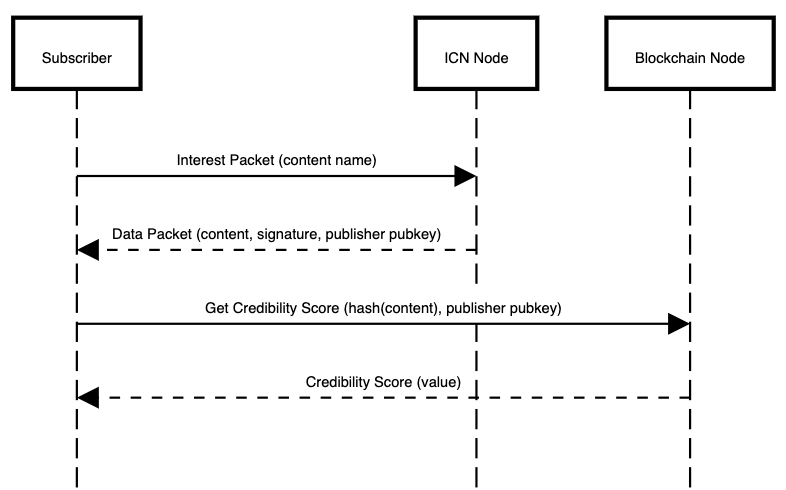
\includegraphics[width=9cm]{img/verifying-flow.png}
\centering
\caption{Flow of fetching and verifying content credibility score}
\label{fig:verifying-flow}
\end{figure} 

The proof-of-time strength is calculated by counting the total number of transactions to the content hash address.

\section{Blockchain structure}
\label{blockchain-structure}
Blocks are fundamental primitives of every blockchain system. A typical block consists of a set of transactions, a Merkle Root \cite{merkle1989certified} that represents the hash of all the transactions, a UNIX timestamp, a hash of the previous block (pointer), a hash of the whole block, and other optional fields\footnote{Blockchains using proof-of-work consensus algorithms also include a nonce field––a proof of the proof-of-work puzzle}.
Blocks are created at some intervals; Bitcoin is designed to produce a new block every 10 minutes on average, Ethereum every 15 seconds, and Stellar every 5 seconds––this value is contractual\footnote{Shorter block creation intervals give faster confirmations, but also speed up the blockchain size growth}. We leverage this feature to achieve a global clock, whereby every block can be interpreted as a clock "tick". By counting the number of "ticks" and multiplying by the "tick" interval, we get an amount of proof-of-time––i.e., a Credibility Score. In Fig. \ref{fig:blockchain-of-claims}, we show an example of three blocks containing proof-of-time claims.
\begin{figure}[h!]
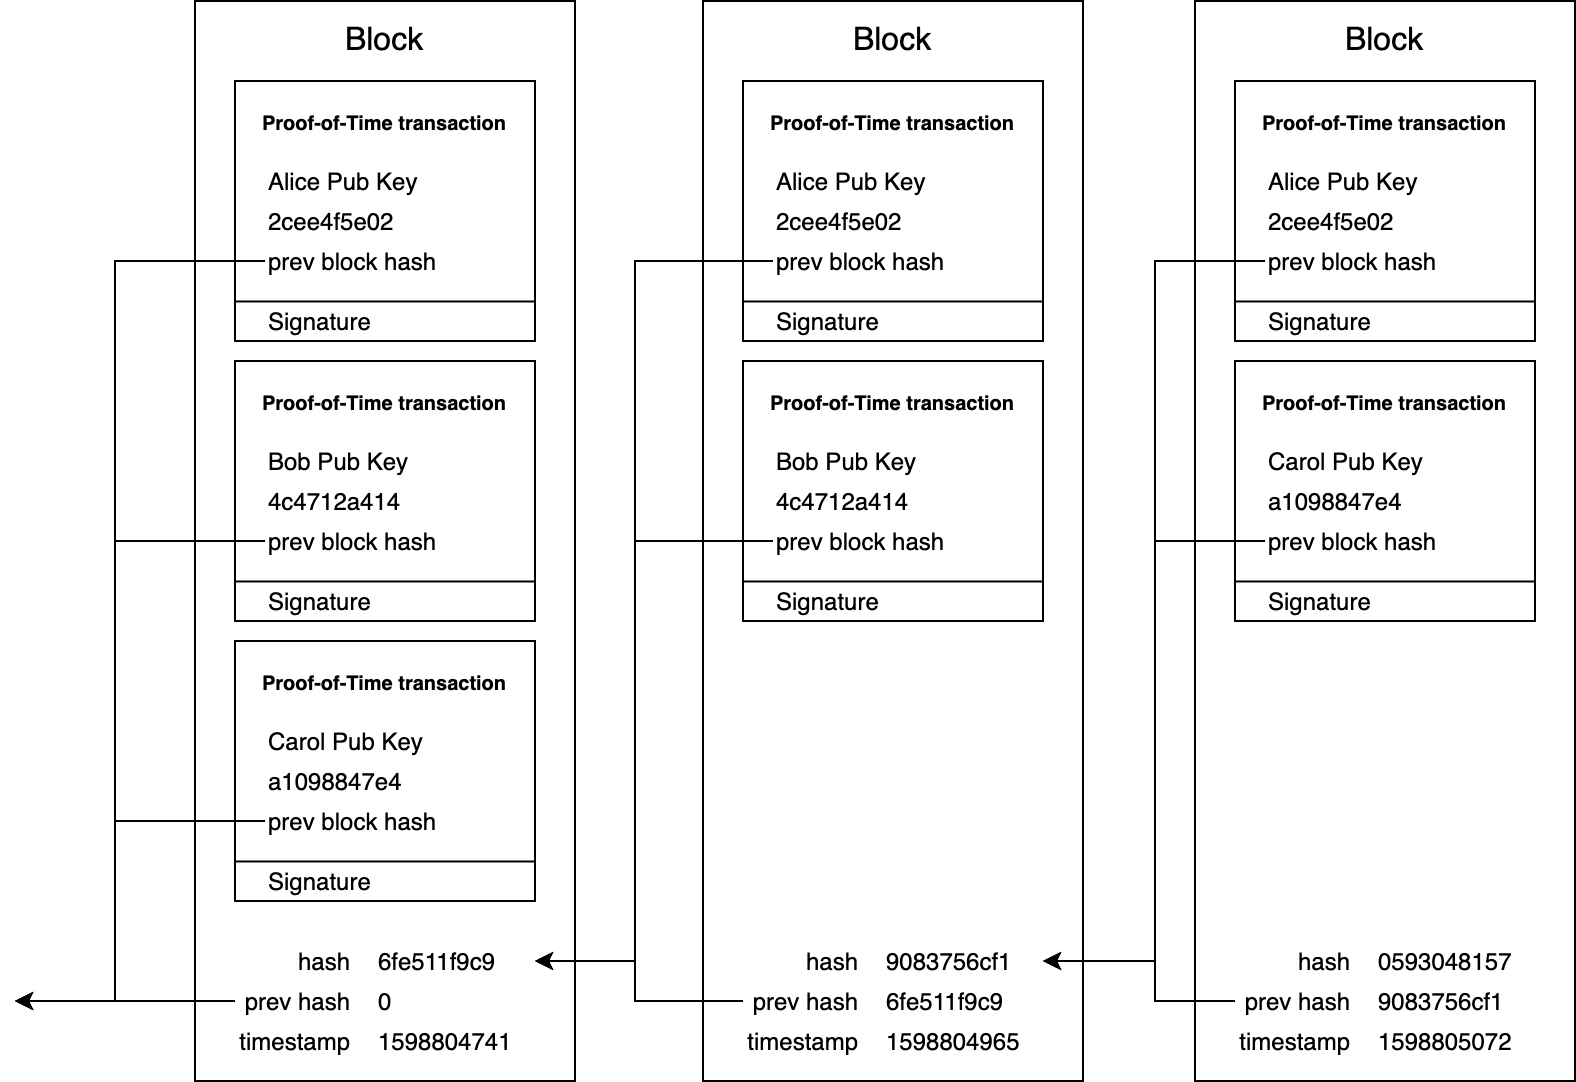
\includegraphics[width=\textwidth]{img/blockchain_of_claims.png}
\centering
\caption{Blockchain of claims}
\label{fig:blockchain-of-claims}
\end{figure} 
We assume that blocks are created with 10-minute intervals, and each content requires a Credibility Score of minimum 20 minutes. Alice first publishes her content to the ICN node getting the hash of the NDO, as shown in Fig. \ref{fig:distribution-flow}, then the proof-of-time transaction is created and published to the blockchain node. After 10 minutes, she again publishes the proof-of-time transaction, and after another 10 minutes she repeats the process. Three publications in a row certify that Alice has had Alice's credentials for at least 20 minutes. Bob was able to publish only two claims, which we consider not enough to trust the content. On the other hand, Carol skipped the second block, which is considered a break in the proof-of-time chain; therefore, counting the proof-of-time for her content starts from the third block. 

\section{Algorithm}
The algorithm used to process new blocks and checking content credibility score is presented in Listing. \ref{listing_process_new_block}. Line 1 defines the state of finalized proof-of-time chains. We allow each content to be authenticated by multiple publishers. Each subscriber can decide which content publisher to trust. Line 2 defines the state of candidate claims–-those that have not broken the proofs chain yet. Each blockchain node, upon receiving a new block, executes the method in line 6; first, it checks if some of the proofs have been broken (are not present in the block), and if so, they are finalized and stored in \verb|stored_claims| (lines 10-14). Then it iterates over transactions present in the block, checks if the \verb|previous_block_hash| matches the actual previous block hash (line 21), then extends the Credibility Score (line 23), and stores the current block hash as a \verb|previous_block_hash|.



%The mechanism can be extended to the "certification services" (discussed in chapter \ref{mitigating-certification-services}) in such a way that not only the publisher can participate in creating proof-of-time claims, but also some set of trusted units that can certify the content trustworthy–––similar how we trust root CA certificates. 

%Attacker who wants to publish bogus content could pre-sign many proof-of-time transactions and then publish them one by one without access to the credentials. To prevent that, we require each publisher to provide the hash of the previous block in the transaction. Since the hash of the block is not deterministic for individual publishers, they cannot pre-sign transactions. Instead, they have to sign the transaction just before sending the transaction to the blockchain.


\begin{lstlisting}[language=Python, caption=Processing a new block, label=listing_process_new_block,float,floatplacement=H]
stored_claims      # { [content-hash] : [publisher_pubkey] : integer }
candidate_claims  # { [content-hash] : [publisher_pubkey] : integer }
previous_block_hash


def process_new_block(block):
    # handle broken proof-of-time chains
    for content_hash in candidate_claims:
        for publisher_pubkey in candidate_claims[content_hash]:
            if (content_hash, publisher_pubkey) not in block.transactions:
                # proofs-of-time chain has been broken, store the length
                stored_claims[content_hash][publisher_pubkey] = 
                    candidate_claims[content_hash][publisher_pubkey]
                delete candidate_claims[content_hash][publisher_pubkey]

    for transaction in block.transactions:
        content_hash = transaction.hash
        publisher_publickey = transaction.publisher_publickey
        previous_block_hash = transaction.previous_block_hash
        # check the previous_block_hash to prevent pre-signed proofs
        if previous_block_hash != previous_block_hash:
            continue
        candidate_claims[content_hash][publisher_publickey] += 1

    previous_block_hash = block.hash


def get_credibility_score(content):
    if stored_claims[content] > candidate_claims[content]:
        return stored_claims[content]
    else:
        return candidate_claims[content]

\end{lstlisting}




\section{Federated Byzantine Agreement}
\label{FBA}
Obviously, the proof-of-work consensus protocol (or any other so-called Nakamoto Consensus protocol, where the leader capable of updating the blockchain is elected in a lottery with the chance of winning depends on the amount of spent resource) is not suitable for the Stolen Credentials problem. However, consensus algorithms in distributed systems have been studied for decades, so there are many protocols to choose from.

We find Federated Byzantine Agreement (FBA)––and its blockchain implementation called Stellar Consensus Protocol (SCP)\cite{mazieres2015stellar} the most suitable for our needs. In contrast to proof-of-work, where computational power dictates the contribution to consensus, FBA is based on a trust model. It becomes a fast, lightweight, and asymptotic resistant\footnote{That is, a node with large computational power does not gain any advantage in the consensus protocol}. Instead, the contribution value is determined by the node trustworthiness, similarly to the GI protocol. A new node joining the network has no contribution to the protocol until someone trusted starts to trust it.

Blockchain, like any other asynchronous distributed system, faces the FLP impossibility trilemma \cite{fischer1985impossibility}, where only two of three properties: Fault Tolerance, Liveness, and Safety, can be achieved. Most systems must be fault tolerant, so the choice is left between Liveness and Safety. Safety guarantees state consistency across all nodes in the network--if nodes do not agree on some transaction, they will not split into two different states, but rather wait until the conflict is resolved. Liveness guarantees that the consensus will always terminate, and the system will always be available to admit new transactions. When a conflict occurs, the ledger is split into two different versions until the conflict is resolved, but in the meantime it can process new transactions. Most of the blockchain protocols choose Liveness, i.e., tolerate temporary partitioning. It is argued that the time of the partitioning is short enough so that users expecting high credibility of the transaction can just wait until the chance of shifting the state is acceptably small\footnote{In proof-of-work, the chance of changing the state of some block diminishes as the chain of blocks attached to this block lengthens}. The conflict settlement is again dictated by the computational power. The state that becomes the ancestor for the next block is considered the winner—-in this way, the system can guarantee permanent availability, even with just one working node. 

Stellar Consensus Protocol (SCP), on the other hand, chooses Safety over Liveness. Once the state has been approved, it cannot be changed. State gets approved when the quorum of the network agree on the proposed state. 
SCP is based on Practical Byzantine fault tolerance (PBFT) \cite{castro1999practical} and extends its functionality by allowing open membership, therefore promoting decentralization. In SCP, each node picks its trusted set of nodes called \textit{quorum slice} (in which it is \textit{ipso facto} a member). The \textit{quorum slice} should be different for each node, but naturally some nodes are more trustworthy and so picked more often for the quorum slices. Transitive trust for all node's \textit{quorum-slice} members, then forms \texitt{quorum}. For any two quorums, there must exist a \textit{quorum-intersection} to prevent network partitioning.

In non-FBA systems, the majority of the nodes determine the consensus decision on some state proposal. Once the proposal gets accepted by a quorum (a majority of the nodes), the rest of the network can be certain that other proposals will fail, because other proposals cannot reach the quorum and because the nodes cannot change their proposals. As a result, the whole network converges to a final decision.
In decentralized systems, where nodes can join and leave at will, the total number of nodes in the network is unknown \texit{a priori}. Therefore, it is hard to determine a majority. Additionally, open systems cannot rely on quantitative majority because it would open them to Sybil attacks\footnote{In this attack, a single entity can join the network as many nodes that to the rest of the network look as independent units, therefore able to force specific decisions}. To solve this problem, FBA introduces a federated voting process that starts locally and expands until it reaches the whole network. The local quorums must overlap with at least one common node to convey the voting decisions across different quorums. This so-called quorum-intersection property guarantees that if one quorum agrees on some value V, the other quorums cannot agree on non-V.

Federated voting starts when some node sends a broadcast to the network announcing a vote on a particular value V. By doing so, the node promises it will never vote against V. Each node sees how other nodes are voting by listening to their broadcass. If a node notices that some quorum of nodes voted on V then, by the definition of quorum, it can be certain that V will eventually be accepted by the whole network. Therefore, it can switch to an \textit{accepting V} state and announce this to the whole network, just as it announced its vote. \textit{accepting V} is stronger than voting--the latter means that the node will never vote for non-V while the former means that \textit{each node in the network} will never accept non-V. When a node notices some quorum of nodes is \textit{accepting V}, it \textit{confirms V}, implying, by the definition of the quorum, that all nodes in the network will eventually have \textit{confirms V}; this ends the process of federated voting.

The problem arises when nodes in a quorum intersection are Byzantine-failed, lying about the decisions made on each quorum. In a SCP whitepaper there is an assumption that the network is configured in such a way that even if the malicious nodes are removed from the network, the quorum-intersection property still holds, otherwise the network halts until the quorum-slices are reconfigured.
We can only expect this property to hold in large real-world networks such as thhe Internet, which we are designing the protocol for.

Another problem with adopting FBA to our use case might be a DoS attack. A malicious publisher may publish a massive amount of proof-of-time transactions successfully, leading to network congestion. Stellar prevents that by introducing the transaction fees. Therefore, the attacker is discouraged by financial means. In our approach we do not want to introduce any payment mechanisms, so other defense mechanisms. DoS is a vital problem in ICN networking as such \cite{gasti2013and}, hence we treat this topic as out-of-scope, referring to the generic solutions for ICN.

Among the various blockchain consensus protocols, not all are suitable as Internet-level protocols that have to run on resource-constrained network devices.
If we consider IoT devices, we can leverage existing research, however, e.g., \cite{salimitari2018survey} suggests that Stellar consensus is not ideal for IoT devices since it is too slow.
Yet in our case the proof-of-time claims are on order of minuter or hours rather tna milliseconds, thus we believe that our protocol is fast enough.
Moreover, there already exists a proposal of a modified FBA algorithm using a virtual voting algorithm \cite{FCPpdf50:online} that can achieve consensus with almost no communication overhead. We find this topic worthy of future work. For now we have settled on FBA in its raw form presented above.



%\section{Transaction throughput}
%Transaction throughput––measured in transactions per second––is one of the biggest problems in the blockchain ecosystem. Bitcoin public network can process up to 7 transactions per second (TPS), Ethereum can process 15TPS and Stellar can process 200TPS. The limitation comes from the practical aspects of the system. If we want the system to be decentralized, we cannot require all nodes in the network to be super-computers, both in processing power and storage capacity. In our case, we design the system for network devices that have limited resources.

%\section{Storage}
%Typically blockchain nodes stores whole blocks that consists of bunch of transactions. Our system does not need to store whole transaction (proof-of-time claims) history. There is no need to do so. After the sequence of proof-of-times is broken, nodes can prune their databases from that transactions, storing only the length of the sequence.